
 
%%\documentclass[sn-nature]{sn-jnl}% Style for submissions to Nature Portfolio journals
%%\documentclass[sn-basic]{sn-jnl}% Basic Springer Nature Reference Style/Chemistry Reference Style
\documentclass[sn-mathphys,Numbered]{sn-jnl}
\usepackage{graphicx}%
\usepackage{multirow}%
\usepackage{amsmath,amssymb,amsfonts}%
\usepackage{amsthm}%
\usepackage{mathrsfs}%
\usepackage[title]{appendix}%
\usepackage{xcolor}%
\usepackage{textcomp}%
\usepackage{manyfoot}%
\usepackage{booktabs}%
\usepackage{algorithm}%
\usepackage{algorithmicx}%
\usepackage{algpseudocode}%
\usepackage{listings}%
\theoremstyle{thmstyleone}%
\newtheorem{theorem}{Theorem}
\newtheorem{proposition}[theorem]{Proposition}% 

\theoremstyle{thmstyletwo}%
\newtheorem{example}{Example}%
\newtheorem{remark}{Remark}%

\theoremstyle{thmstylethree}%
\newtheorem{definition}{Definition}%

\raggedbottom

\begin{document}

\title[Article Title]{Cold Ideal Fermi Gas }

%%=============================================================%%
%% Prefix	-> \pfx{Dr}
%% GivenName	-> \fnm{Joergen W.}
%% Particle	-> \spfx{van der} -> surname prefix
%% FamilyName	-> \sur{Ploeg}
%% Suffix	-> \sfx{IV}
%% NatureName	-> \tanm{Poet Laureate} -> Title after name
%% Degrees	-> \dgr{MSc, PhD}
%% \author*[1,2]{\pfx{Dr} \fnm{Joergen W.} \spfx{van der} \sur{Ploeg} \sfx{IV} \tanm{Poet Laureate} 
%%                 \dgr{MSc, PhD}}\email{iauthor@gmail.com}
%%=============================================================%%

\author[1]{\fnm{}\sur{Cheng Tao Yang}}%\email{iauthor@gmail.com}

\author[1,2]{\fnm{} \sur{Martin Formanek}}%\email{iiauthor@gmail.com}
%\equalcont{These authors contributed equally to this work.}

\author[1]{\fnm{} \sur{Johann Rafelski}}%\email{iiiauthor@gmail.com}
%\equalcont{These authors contributed equally to this work.}

\affil[1]{\orgdiv{Department of Physics}, \orgname{The University of Arizona}, \city{Tucson}, \state{Arizona}, \postcode{85721}, \country{USA}}

\affil[2]{\orgdiv{ELI Beamlines Facility}, \orgname{The Extreme Light Infrastructure ERIC}, \orgaddress{ \postcode{252 41}, \city{Dolni Brezany}, \country{Czech Republic}}}

%\affil[3]{\orgdiv{Department}, \orgname{Organization}, \orgaddress{\street{Street}, \city{City}, \postcode{610101}, \state{State}, \country{Country}}}

%%==================================%%
%% sample for unstructured abstract %%
%%==================================%%

\abstract{
We present a novel form of Fermi distribution allowing to evaluate the properties of Fermi gas at low temperature.
%This novel formulation of Fermi distribution extends the understanding of physics beyond the conventional zero-temperature limit.
}

%have identified an innovative approach to express the form of the Fermi distribution, which can be use at low temperatures physics where the Fermi gas remain degenerate and their special feature persist. This novel formulation of Fermi distribution extends the understanding of physics beyond the conventional zero-temperature limit.}


\keywords{Fermi distribution, Low temperature Fermi gas}

%%\pacs[JEL Classification]{D8, H51}

%%\pacs[MSC Classification]{35A01, 65L10, 65L12, 65L20, 65L70}

\maketitle

\section{Introduction}\label{sec1}
In the extreme limit $T\rightarrow0$, the Fermi-Dirac distribution becomes very simple: a state is either filled or empty. We have
\begin{align}\label{f_old}
f&=\frac{1}{e^{(E-\tilde{\mu})/T}+1}=\left\{\begin{array}{c}1,\,\,\,\mathrm{for}\,\,\,{E}<\tilde{\mu} \\0,\,\,\,\mathrm{for}\,\,\, {E}>\tilde{\mu}\end{array}\right.
\end{align}
The energy of the last filled state is called the Fermi energy and is denoted as $E_F$. It is the value of the chemical potential at zero temperature $T=0$, i.e., $E_F=\tilde\mu(T = 0)$. In Fig.~\ref{Electron_001} we plot the Fermi-distribution of electron as a function of energy where the parameters are given by $T=0.012\,\mathrm{MeV}$ and chemical potential $\tilde\mu=0.461$ MeV.

%~~~~~~~Figure~~~~~~~~~~~~~~~~~~~~~~~~~~~~~~~~~~~~~
\begin{figure}[h]
\begin{center}
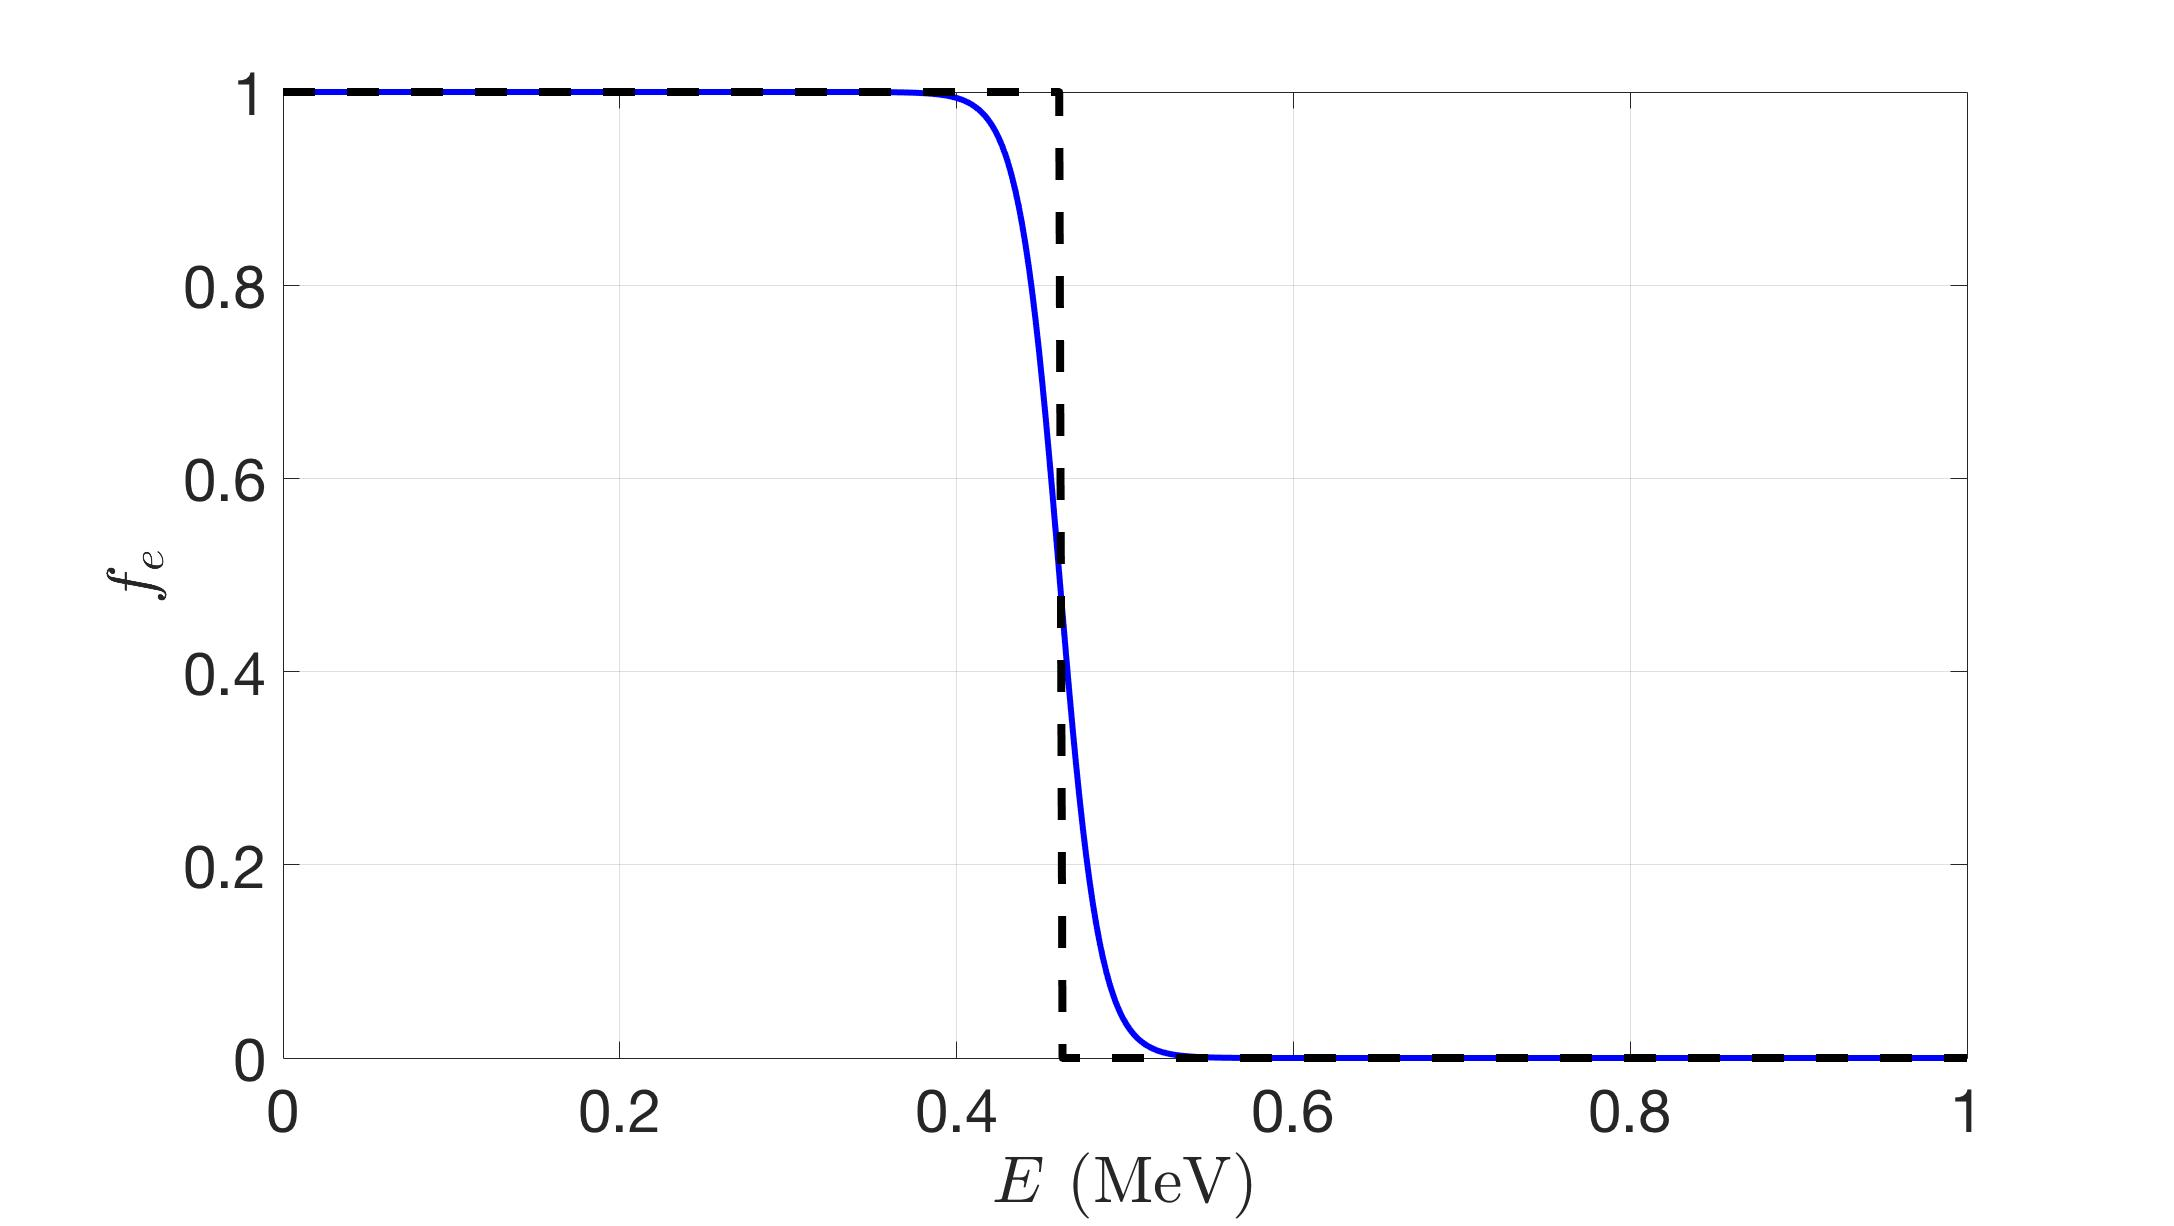
\includegraphics[width=0.9\textwidth]{./plot/Electron_distribution001}
\caption{The Fermi-distribution  as a function of energy where the parameters are given by $T=0.012\,\mathrm{MeV}$ and chemical potential $\tilde\mu=0.461$ MeV.}
\label{Electron_001}
\end{center}
\end{figure}
%~~~~~~~~~~~~~~~~~~~~~~~~~~~~~~~~~~~~~~~~~~~~~~~~~~




%%%%%%%%%%%%%%%%%%%%%%%%%%%%%%%%%%%%%%%%%%%%
\section{Exact finite temperature correction to Fermi distribution}\label{NewFermi}

\subsection{A novel form of Fermi distribution}
We have empirically identified the following novel way to state the form of the Fermi distribution. We obtained this form seeking to carry out cosmological computations involving shift in behavior from high to very low-temperature physics. 
\begin{align}\label{NFF1}
f&\equiv \frac{1}{e^{ (E-\tilde\mu)/T} +1}\notag\\
&=\Theta(\tilde\mu - E) +  e^{ - |E-\tilde\mu|/T }
\; \left[\frac{1}{2}\mathrm{sgn}\left({E-\tilde\mu}\right) 
 +\frac{1}{2}\tanh\left(\frac{E-\tilde\mu}{2T}\right)\right]
\end{align}
Note also that the expression in square bracket is a modified form of the sign-function which interpolates between $-1,+1$ for $x\pm \infty$ with a half-unit-sized jump at origin.  We note  that the right hand side (RHS) of Eq.\,(\ref{NFF1}) comprises several non-analytical functions also called distributions. On first sight it is hard to believe that  these   cancel to create the analytical Fermi function format seen on the left hand side (LHS). In the following, we will demonstrate that both sides equal to each other.


\subsection{Mathematical proof}
To demonstrate the novel form of Fermi distribution, we will use the properties of singular functions as follows: 
\begin{align}\label{NFF2a}
\mathrm{sgn}(x)%\equiv \frac{d|x|}{dx}
\equiv  \frac{|x|}{x}\equiv \frac{x}{|x|}\;,
   \quad \mathrm{sgn}(0)=0,\qquad
 \mathrm{sgn}(x)=2\Theta(x)-1\;,
 \end{align}
 and for the step function we use here
 \begin{align}
\label{NFF2c}
 \Theta(x)+\Theta(-x)=1\;,\qquad
 \Theta(0)=1/2\;.
 \end{align}
We will need just one complicated expression:
\begin{equation}\label{NFFa1}
\mathrm{sgn}^{2}(x)\sinh(x)=\sinh(x)\;.
 \end{equation}
This is so since $\sinh(x)$  vanishes  at $x=0$ thus we need not worry what value to assign to $\mathrm{sgn}^{2}(x)$ at $x=0$.  

To shorten the notations we define variables as follow
\begin{align}
x^\prime=E-\tilde\mu,\qquad A = \frac{x^\prime}{T}= \frac{E-\tilde\mu}{T}
\end{align}
with these new notations the Fermi function can be written as
\begin{align}
f=\Theta(-x^\prime)+e^{-|A|}\left[\frac{1}{2}\mathrm{sgn}\left(x^\prime\right) 
 +\frac{1}{2}\tanh\left(A\right)\right]
\end{align}
Replacing the step function and exponential function as  follow
 \begin{align}\label{NFF4}
&\Theta(-x^\prime)=\frac 1 2 (1-\mathrm{sgn}(x^\prime))\;,\\ 
&e^{-|A|}=\cosh|A|-\sinh|A|=\cosh A- \mathrm{sgn}(x^\prime)\sinh A\;.
\end{align}
then the Fermi distribution function becomes
\begin{align}
f=\frac{1}{2} &+\left[\cosh {A}- \mathrm{sgn}(x^\prime)\sinh{A} -1\right]\frac{1}{2} \mathrm{sgn}(x^\prime)\notag\\
 &\qquad\qquad\qquad+\left[\cosh{A}- \mathrm{sgn}(x)\sinh{A} \right]\frac{1}{2}\tanh{(A/2)}\;.
\end{align}
Using the properties of singular function  Eq.\,(\ref{NFFa1}), the distribution function can be written as
\begin{align}
f=f_R+f_I
\end{align}
where $f_R$ and $f_I$ represent regular and irregular part of distribution respectively. We have
\begin{align}\label{NFF5a}
 f_R=& \frac{1}{2}\left(1-\sinh A +\cosh A \tanh (A/2)\right) \\
 f_I=& \mathrm{sgn}(x) \frac{1}{2} \left(\cosh A-1 - \sinh A \tanh (A/2)\right)
 \label{NFF5b}
\end{align}

For the irregular part $f_I$, we use the properties of hyperbolic functions
\begin{align}
\cosh A-1= 2\sinh^2(A/2), \qquad\sinh A=2 \sinh(A/2) \cosh(A/2)
\end{align}
then it can be written as
\begin{align}
f_I&=\mathrm{sgn}(x) \frac{1}{2} \left[ 2\sinh^2(A/2) - 2 \sinh(A/2) \cosh(A/2) \tanh (A/2)\right]\\
&=\mathrm{sgn}(x) \frac{1}{2}\left[2\sinh^2(A/2)-2\sinh^2(A/2)\right]\\
&=0
\end{align}
we show that the irregular part $f_I$ vanishes as an identity. On the other hand, the regular part $f_R$ can be simplified as below:
\begin{align}
f_R&=\frac{1}{2}\left[1-\frac{1}{2}\left(e^A-e^{-A}\right)+\frac{1}{2}\left(e^A+e^{-A}\right)\frac{e^A-1}{e^A+1}\right]\\
&=\frac{1}{2(e^A+1)}\left[\left(e^A+1\right)-\frac{1}{2}\left[\left(e^A+1\right)\left(e^A-e^{-A}\right)-\left(e^A-1\right)\left(e^A+e^{-A}\right)\right]\right]\\
&=\frac{1}{2(e^A+1)}\left[\left(e^A+1\right)-\left(e^A-1\right)\right]\\
&=f
\end{align}


Finally, we consider the LHS and RHS of Eq.\,(\ref{NFF1}) at $x=0$. With the singular function properties as given we see that at $x=0$ both LHS and RHS of Eq.\,(\ref{NFF1}) are equal to $1/2$ and in the first derivative of the  RHS the two $\delta(x)$-terms 
\begin{align}\label{NFF1b}
\frac{d\Theta(\tilde\mu-E)}{dE}=-\delta(\tilde\mu-E)\;,\qquad 
\frac{d\mathrm{sgn}(E -\tilde\mu)}{dE}=-2\delta(E-\tilde\mu)\;, 
 \end{align}
cancel exactly as required, since there is no $\delta(x)$ on LHS. This encourages us to believe that all of singular expressions cancel. This completes the demonstration of the exact validity of  Eq.\,(\ref{NFF1}). 

\subsection{Numerical illustration}
In Fig.~\ref{Fermi_Checking} we plot the exact Fermi-distribution (LHS of Eq.~(\ref{NFF1}) with solid lines and novel form of Fermi-distribution (RHS of Eq.~(\ref{NFF1})) with dashed lines as a function of energy with different parameters. It demonstrate that 
LHS and RHS of Eq.~(\ref{NFF1}) are equivalent to each other numerically.

%~~~~~~~Figure~~~~~~~~~~~~~~~~~~~~~~~~~~~~~~~~~~~~~~~~~~~~~~~~~~~~~~~~~~~~~~~~~~~~~~~~~~~~~~~~~~~~~
\begin{figure}[h]
\begin{center}
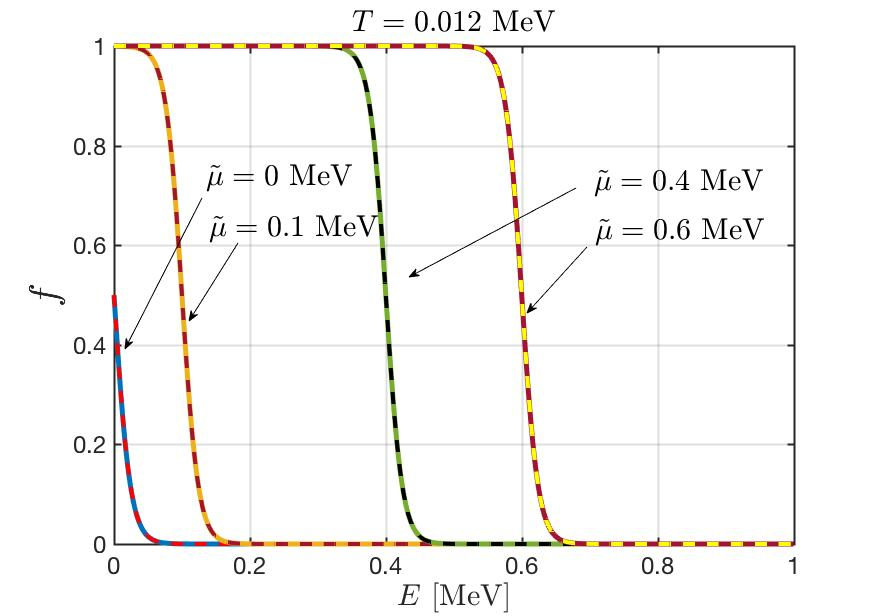
\includegraphics[width=0.5\textwidth]{./plot/Fermi_novel_001}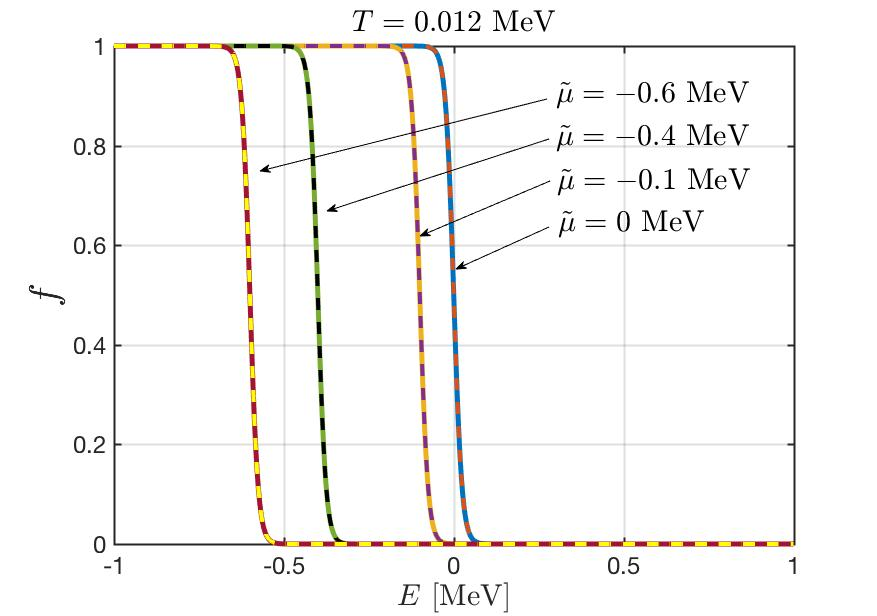
\includegraphics[width=0.5\textwidth]{./plot/Fermi_novel_002}
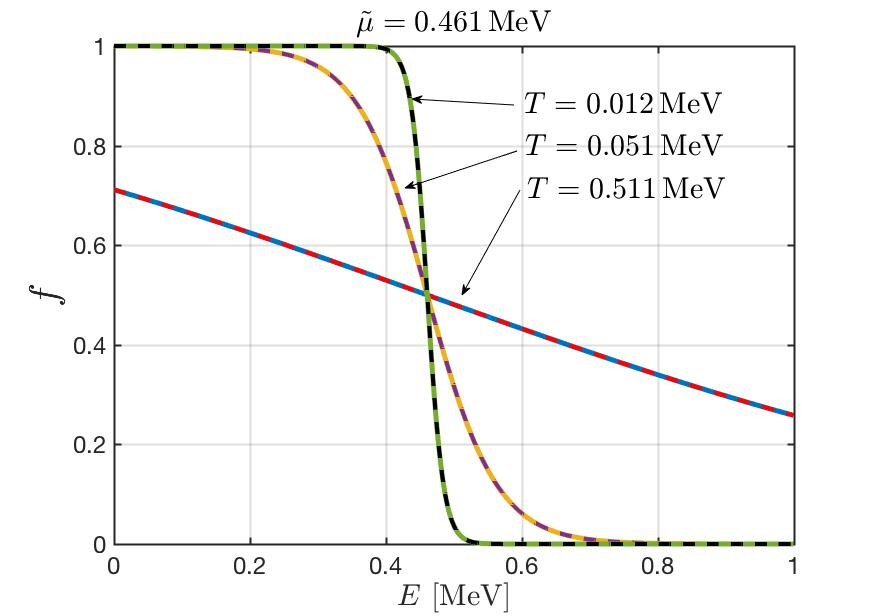
\includegraphics[width=0.5\textwidth]{./plot/Fermi_novel_003}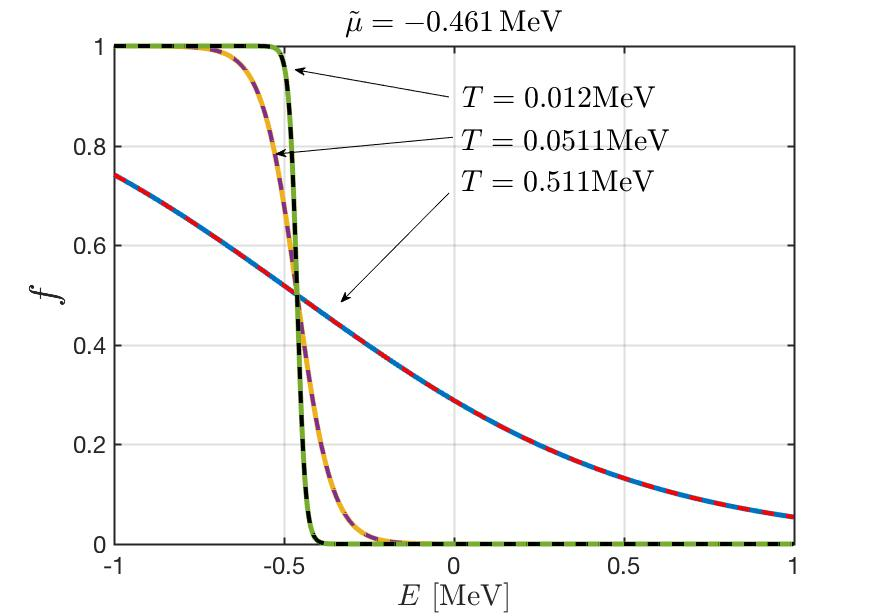
\includegraphics[width=0.5\textwidth]{./plot/Fermi_novel_004}
\caption{The exact Fermi-distribution (LHS of Eq.~(\ref{NFF1}) with solid lines and novel form of Fermi-distribution (RHS of Eq.~(\ref{NFF1})) with dashed lines as a function of energy with different parameters.Top: we compare the RHS and LHS of Eq.~(\ref{NFF1}) with different chemical potential: $\tilde\mu=0, \pm0.1, \pm0.4\,\pm0.6\, \mathrm{MeV}$ at temperature $T=0.012\,\mathrm{MeV}$. Bottom: the Fermi distribution with different temperatures $T=0.511, 0.0511, 0.012\,\mathrm{MeV}$ for chemical potential $\tilde\mu=\pm0.461\,\mathrm{MeV}$.}
\label{Fermi_Checking}
\end{center}
\end{figure}
%~~~~~~~~~~~~~~~~~~~~~~~~~~~~~~~~~~~~~~~~~~~~~~~~~~~~~~~~~~~~~~


%%%%%%%%%%%%%%%%%%%%%%%%%%%%%%%%%%%%%%%%%%%%%%%%%%%%%%%%%%%%%%%%%%%%%%%%%

\section{Partition function and application}\label{NumericalResult}
\subsection{Application: The speed of sound}

In previous section we demonstrate that the Fermi-distribution can be written into a novel form Eq.~(\ref{NFF1}). To illustrate the benefits of our innovative Fermi distribution function in practical applications, it is convenient to introduce the partition function and consider the physical quantity the velocity of sound as a example.

In general, the partition function of Fermi gas can be written as
\cite{letessier_rafelski_2023}
\begin{align}
\ln{Z}&={gV}\int \frac{d^3p}{(2\pi)^3}\ln(1+\gamma\lambda e^{-\beta E})
\end{align}
where $V$ is the volume, $g$ is the degeneracy factor,$\beta=1/T$,  $\gamma$ is the fugacity parameter and $\lambda=e^{\mu/T}$ is related to chemical potential $\mu$. 

We can simplify the partition function via integrating by parts, we obtain
\begin{align}
\ln{Z}&=gV\frac{\beta}{3}\int \frac{d^3p}{(2\pi)^3}p\frac{\partial E}{\partial p}\frac{1}{\gamma^{-1}\lambda^{-1}e^{\beta E}+1}\notag\\
&=\frac{gV}{3T}\int\frac{d^3p}{(2\pi)^3}\frac{p^2}{E}\frac{1}{e^{(E-\tilde\mu)/T}+1}
=\frac{gV}{3T}\int \frac{d^3p}{(2\pi)^3}\frac{p^2}{E}f
\end{align}
where we introduce the the general chemical potential $\tilde\mu$ as follow
\begin{align}
\tilde\mu=\mu+T\ln\gamma.
\end{align}
By definition the speed of sound $v_s$ can be written as
\begin{align}\label{Def_sound}
v^{-2}_s\equiv\left(\frac{d\epsilon}{dP}\right)_{S,N},
\end{align}
where $\epsilon$ is the energy density and $P$ is the pressure of Fermi gas. When taking the partial differentials, the subscripts $S$ and $N$ denote the fixed entropy and number of particles, respectively. To evaluate the speed of sound from partition function, we consider the pressure  first, we have
\begin{align}
P&=T\frac{\partial}{\partial V} \ln{Z}\notag\\
&=\frac{1}{3}\left[g\int\!\!\frac{d^3p}{(2\pi)^3}\left(E-\frac{m^2}{E}\right)f\right]=\frac{1}{3}\left[g\int\!\!\frac{d^3p}{(2\pi)^3}E\,f-g\int\!\!\frac{d^3p}{(2\pi)^3}\frac{m^2}{E}\,f\right]
\end{align}
and it can be written as
\begin{align}
3P=\epsilon-g\int\frac{d^3p}{(2\pi)^3}\frac{m^2}{E}\,f,\qquad \epsilon=g\int\frac{d^3p}{(2\pi)^3}E\,f.
\end{align}
In this case, by the definition Eq.~(\ref{Def_sound}) the speed of sound can be written as
\begin{align}\label{Sound_eq}
&v^{-2}_s=3+\frac{dT}{dP}\frac{d}{dT}\left[g\int\!\!\frac{d^3p}{(2\pi)^3}\frac{m^2}{E}\,f\right]=3\left[1+\frac{M}{N}\right],
\end{align}
where the functions $M$ and $N$ are defined as
\begin{align}
\label{M_eq}
&M\equiv g\int\!\!\frac{d^3p}{(2\pi)^3}\frac{m^2}{E}\,\frac{df}{dT}=\frac{g}{2\pi^2}\int_m^\infty\!\!dE \left(m^2\sqrt{E^2-m^2}\right)\frac{df}{dT}\,,\\
\label{N_eq}
&N=g\int\!\!\frac{d^3p}{(2\pi)^3}\frac{p^2}{E}\,\frac{df}{dT}=\frac{g}{2\pi^2}\int_m^\infty\!\!dE \left({E^2-m^2}\right)^{3/2}\frac{df}{dT}.
\end{align}
From Eq.~(\ref{Sound_eq}) we see for relativistic Fermi gas $m\to 0$, we obtain the standard value for the speed of sound $v_s=1\sqrt{3}$. For the nonrelativistic limit $m\gg T$, we can take the Boltzmann distribution in the calculation, then the speed of sounds becomes
\begin{align}
\left(\frac{1}{v^B_s}\right)^2=3+\frac{m}{T}\frac{K_2(m/T)}{K_3(m/T)}\longrightarrow\left(3+\frac{m}{T}\right),\qquad \mathrm{for}\quad m\gg T
\end{align}
where $K_2$ and $K_3$ are the 2nd and 3rd order of Bessel function, and we take the nonrelativistic limit $m\gg T$ for the ratio between Bessel functions to obtain the nonrelativistic speed of sounds for Fermi gas.

%~~~~~~~Figure~~~~~~~~~~~~~~~~~~~~~~~~~~~~~~~~~~~~~
\begin{figure}[h]
\begin{center}
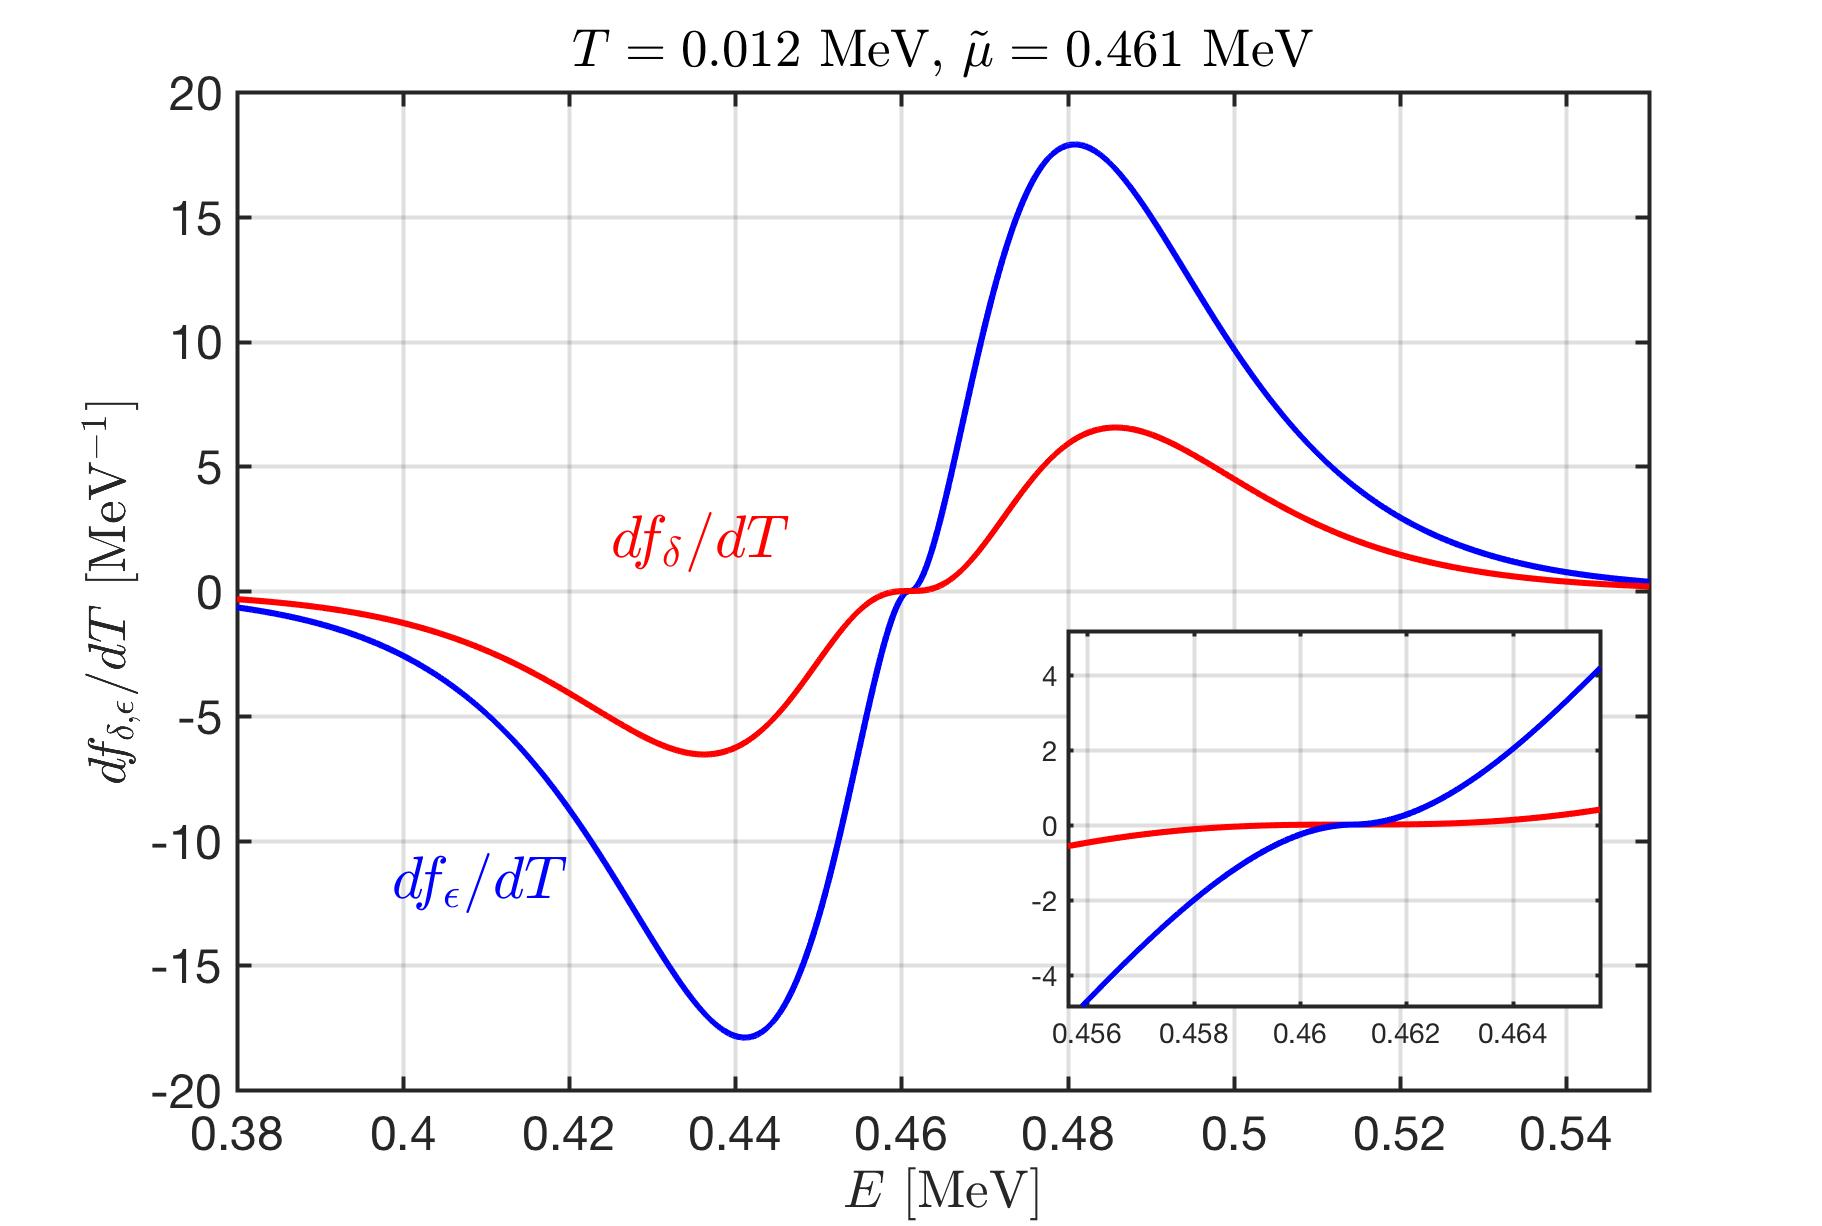
\includegraphics[width=0.9\textwidth]{./plot/NewFermi_dfdT002}
\caption{The $df_\delta/dT$ and $df_\epsilon/dT$ as a function of energy where the parameters are given by $T=0.012\,\mathrm{MeV}$ and chemical potential $\tilde\mu=0.461$ MeV.}
\label{dfdT_fig}
\end{center}
\end{figure}
%~~~~~~~~~~~~~~~~~~~~~~~~~~~~~~~~~~~~~~~~~~~~~~~~~~
%~~~~~~~Figure~~~~~~~~~~~~~~~~~~~~~~~~~~~~~~~~~~~~~
\begin{figure}[h]
\begin{center}
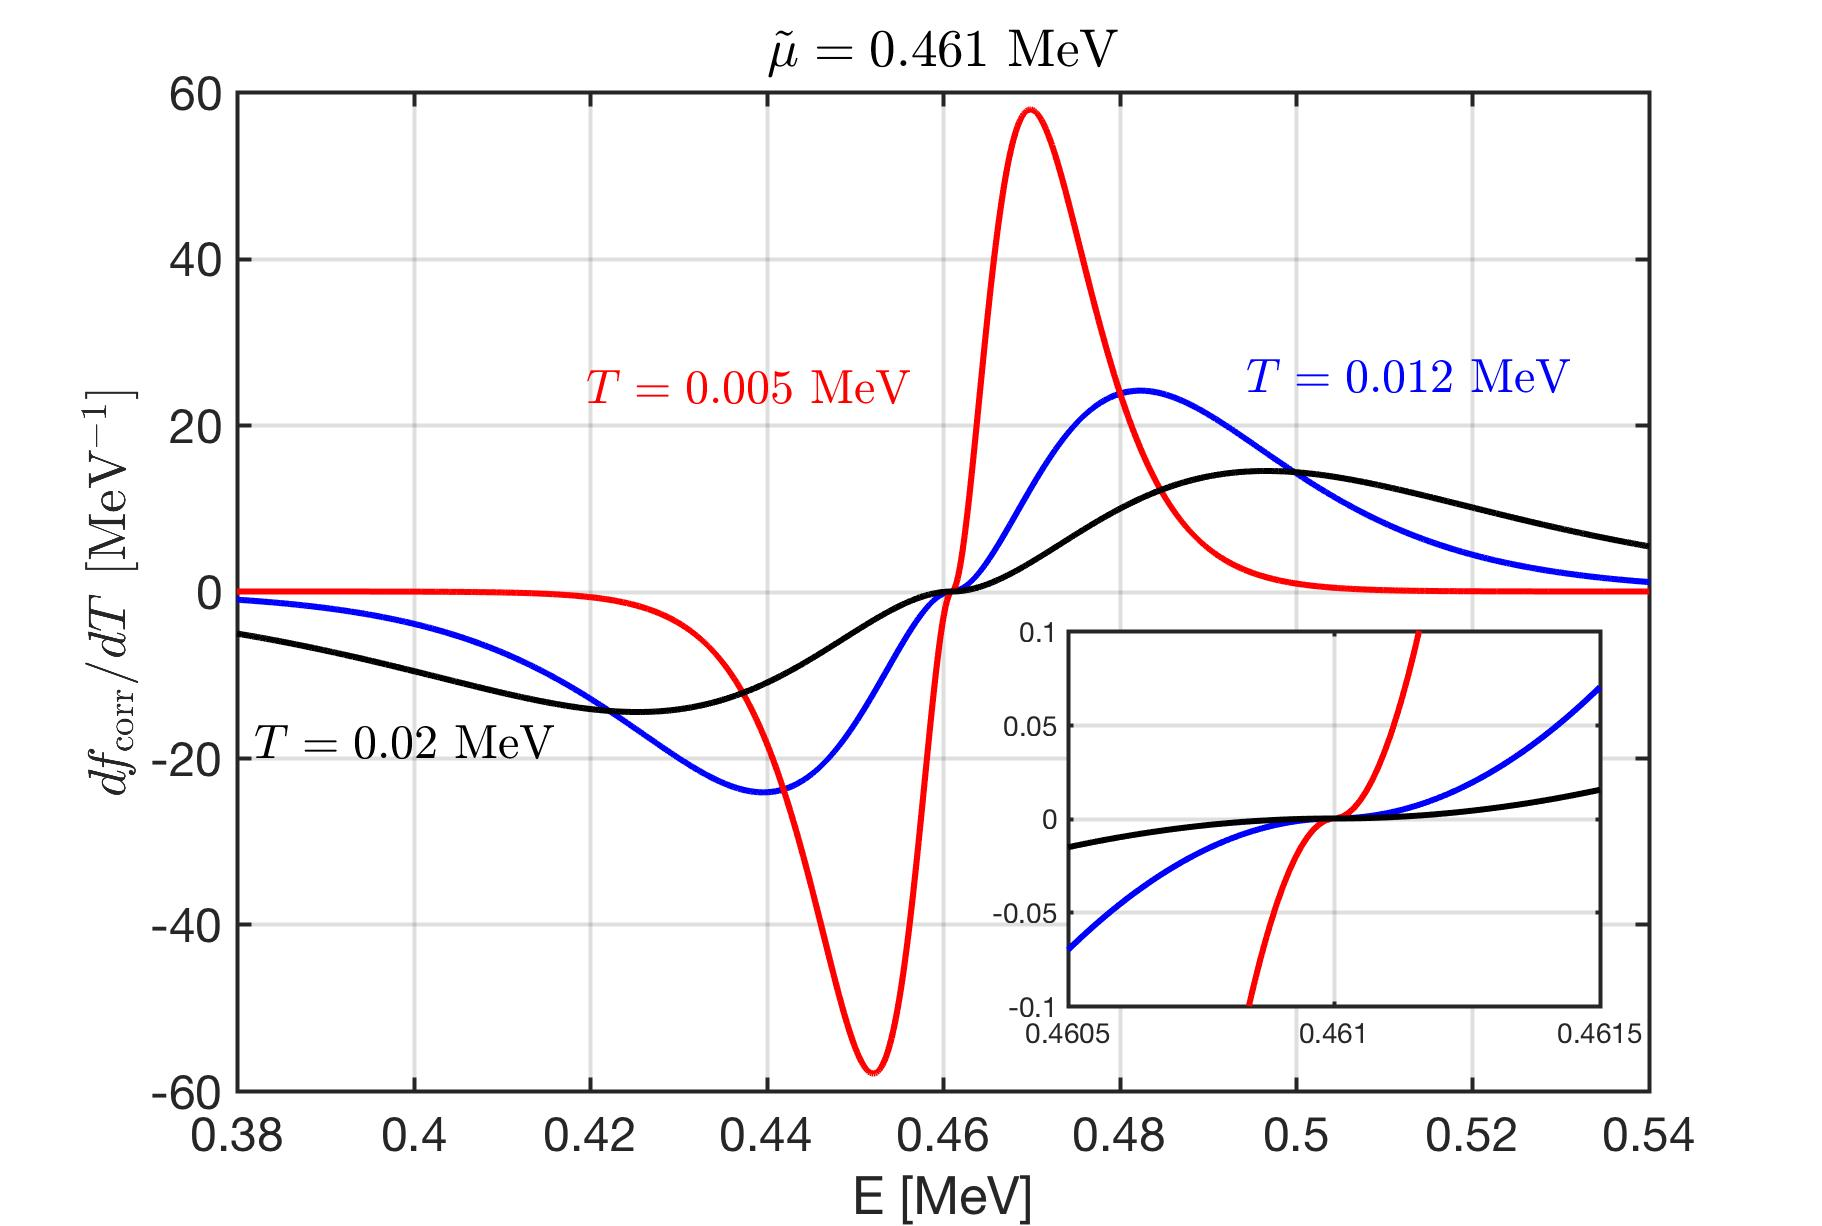
\includegraphics[width=0.9\textwidth]{./plot/NewFermi_dfdT_tot}
\caption{
The $df_\mathrm{corr}/dT$ as a function of energy with chemical potential $\tilde\mu=0.461$ MeV.The bule line represents the temperature $T=0.012$ MeV, red line label $T=0.005$ MeV, and black line is $T=0.02$ MeV.}
\label{dfdT_tot_fig}
\end{center}
\end{figure}
%~~~~~~~~~~~~~~~~~~~~~~~~~~~~~~~~~~~~~~~~~~~~~~~~~~

The property of speed of sound $v_s$ depends on the Fermi distribution $df/dT$. To illustrate the benefits of our novel Fermi distribution
function in calculation of speed of sound, it is convenient to rewrite the Fermi-function as 
\begin{align}
f=f_{\mathrm{cold}} +f_\mathrm{corr}.
\end{align}
where the function $f_{\mathrm{cold}}$, $f_\mathrm{corr}$ is defined as
\begin{align}
&f_{\mathrm{cold}}=\Theta(\tilde\mu-E),\\
&f_\mathrm{corr}=\frac{1}{2}\,e^{-|E-\tilde\mu|/T}\left[\frac{(E-\tilde\mu)}{|E-\tilde\mu|}+\tanh\bigg(\frac{E-\tilde\mu}{2T}\bigg)\right],
\end{align}
where $f_{cold}$ corresponds to the Fermi distribution with zero temperature limit $T\to0$, and $f_\mathrm{corr}$ corresponds to the distribution beyond the conventional zero-temperature limit.
In this case, the non-zero derivatives of the Fermi functions  with respect to the temperature can be written as
\begin{align}
\frac{df_{\mathrm{corr}}}{dT}=\frac{df_\delta}{dT}+\frac{df_\epsilon}{dT}
\end{align}
where the functions ${df_\delta}/{dT}$ and $df_\epsilon/dT$ are defined as
\begin{align}
\label{dfdT001}
&\frac{df_\delta}{dT}=\frac{(E-\tilde\mu)}{2T^2}e^{-|E-\tilde\mu|/T}\tanh^2\bigg(\frac{E-\tilde\mu}{2T}\bigg),\\
\label{dfdT002}
&\frac{df_\epsilon}{dT}=\frac{|E-\tilde\mu|}{T^2}e^{-|E-\tilde\mu|/T}\!\tanh\bigg(\frac{E-\tilde\mu}{2T}\bigg).
\end{align}

%~~~~~~~Figure~~~~~~~~~~~~~~~~~~~~~~~~~~~~~~~~~~~~~
\begin{figure}[h]
\begin{center}
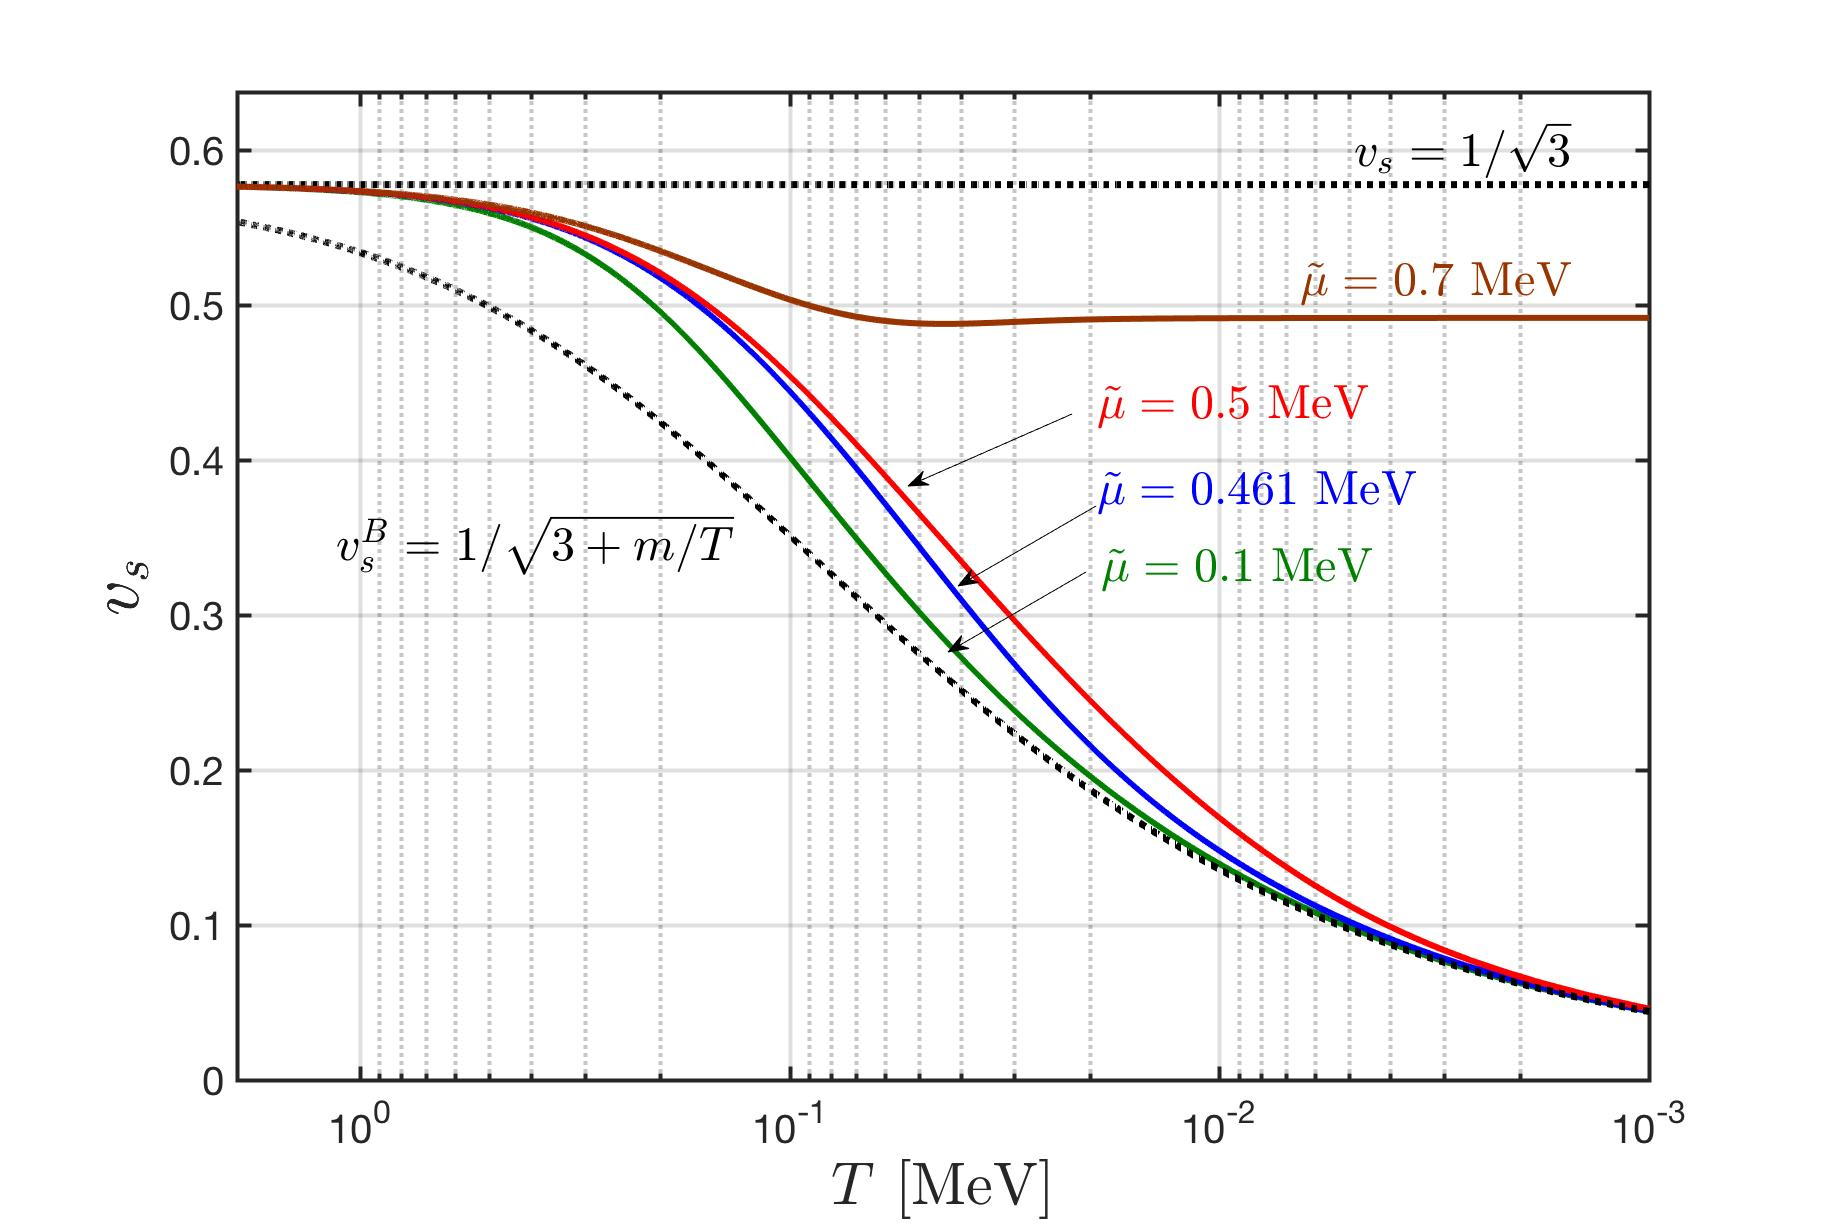
\includegraphics[width=0.9\textwidth]{./plot/SoundSpeed002}
\caption{
The speed of sound $v_s$ for electron ($m=0.511$ MeV) as a function of temperature with different chemical potentials. The horiztional black dotted line represents the relativistic limit $v_s=1/\sqrt{3}$ and the lower black dotted line is the speed of sound in Boltzmann limit $v_s^B=1/\sqrt{3+m/T}$.}
\label{SoundSpeed_fig}
\end{center}
\end{figure}
%~~~~~~~~~~~~~~~~~~~~~~~~~~~~~~~~~~~~~~~~~~~~~~~~~~

In Fig.~\ref{dfdT_fig} we plot $df_\delta/dT$ and $df_\epsilon/dT$ as a function of energy where the parameters are given by $T=0.012\,\mathrm{MeV}$ and chemical potential $\tilde\mu=0.461$ MeV. It shows that both $df_\delta/dT$ and $df_\epsilon/dT$ equal to zero when $E=\tilde\mu$. This is truth for all the higher-order derivative of Fermi function with respect to temperature, which can be verified by taking the derivative of Eq~(\ref{f_old}) with temperature. In Fig.~\ref{dfdT_tot_fig} we plot $df_\mathrm{corr}/dT$ at $\tilde\mu=0.461$ MeV as a function of energy with varying temperatures. It shows that for lower temperature the function $df_\mathrm{corr}/dT$ become like the delta function around the energy $E=\tilde\mu$.

Substituting Eq.~(\ref{dfdT002}) and Eq.~(\ref{dfdT002}) into Eq.~(\ref{M_eq}) and Eq.~(\ref{N_eq}) then we can obtain the speed of sounds numerically. In Fig.~\ref{SoundSpeed_fig} we plot the speed of sound $v_s$ as a function of temperature with different chemical potentials. By using our new form of Fermi function to evaluate the speed of sound, it shows the correct limit for both high and low temperatures. 




%%%%%%%%%%%%%%%%%%%%%%%%%%%%%%%%%%%%%%%%%%%%%%%%%%%%%%%%%%%%%%%%%
\subsection{Application: Magnetization}
Considering the partition function of $e^\pm$ gas in a uniform magnetic field $B$ pointing along the $z$-axis, we have
\begin{align}
\ln\mathcal{Z}_{tot}=eBV\sum_{s=\pm1}\sum_{j=0}^\infty\int^\infty_{-\infty} \!\!dp_z\bigg[\ln\left(1+e^{-\beta(E_{j,s}-\mu_e)}\right)+\ln\left(1+e^{-\beta(E_{j,s}+\mu_e)}\right)\bigg],
\end{align}
where $\beta=1/T$, $\mu_e$ is the chemical potential of electron, and the electron(positron) energy $E_{j,s}$ can be written as
\begin{align}
E_{j,s}&=\sqrt{m^2_e+p^2_z+2eB\left(j+\frac{1}{2}+\frac{g}{4}s\right)},\qquad s=\pm1,\qquad j=0,1,2,\dots
\end{align}
and $\mu_B$ is the magnetic moment. 

Considering the integral over $dp_z$ we can simplify the integration by integrating by part, we have
\begin{align}
&\int^\infty_{-\infty} \!\!dp_z\bigg[\ln\left(1+e^{-\beta(E_{j,s}-\mu_e)}\right)+\ln\left(1+e^{-\beta(E_{j,s}+\mu_e)}\right)\bigg]\notag\\
&=2\bigg[\int_0^\infty\!\!dp_z\ln\left(1+e^{-\beta(E_{j,s}-\mu_e)}\right)+\int_0^\infty\!\!dp_z\ln\left(1+e^{-\beta(E_{j,s}+\mu_e)}\right)\bigg]\\
&=2\bigg[\beta\int_0^\infty\!\!dp_z p_z\frac{\partial E_{j,s}}{\partial p_z}\frac{1}{e^{\beta(E_{j,s}-\mu_e})+1}+\beta\int_0^z\!\!dp_z p_z\frac{\partial E_{j,s}}{\partial p_z}\frac{1}{e^{\beta(E_{j,s}+\mu_e})+1}\bigg]\\
&=2\beta\int_0^\infty\!\!dp_z \frac{p_z^2}{E_{j,s}}\left[\frac{1}{e^{\beta(E_{j,s}-\mu_e})+1}+\frac{1}{e^{\beta(E_{j,s}+\mu_e})+1}\right]
\end{align}

Then the partition function of $e^\pm$ plasma in a uniform magnetic field $B$ can be written as
\begin{align}
\ln\mathcal{Z}_{tot}&=eBV\sum_{s=\pm1}\sum_{j=0}^\infty2\beta\int_0^\infty\!\!dp_z \frac{p_z^2}{E_{j,s}}\left[\frac{1}{e^{\beta(E_{j,s}-\mu_e})+1}+\frac{1}{e^{\beta(E_{j,s}+\mu_e})+1}\right]\\
&=eBV\sum_{s=\pm1}\sum_{j=0}^\infty2\beta\int_0^\infty\!\!dp_z \frac{p_z^2}{E_{j,s}}\bigg[f_{e^-}+f_{e^+}\bigg].
\end{align}
Considering the case {\color{blue}$g=2$}, then we have
\begin{align}
 &E_{j,+}=\sqrt{{m}_e^2+p^2_z+2eB\left(j+1\right)}\longrightarrow E_{n}=\sqrt{{m}_e^2+p^2_z+2eBn},\qquad n=1,2,3,\dots\\
 &E_{j,-}=\sqrt{{m}_e^2+p^2_z+2eB\left(j\right)}\longrightarrow E_{n}=\sqrt{{m}_e^2+p^2_z+2eBn},\qquad n=0,1,2,3,\dots
\end{align}
where we change the index from $j$ to $n$. In this case, the partition function of $e^\pm$ plasma can be written as
\begin{align}
\ln\mathcal{Z}_{tot}&=V(2eB\beta) \bigg[ \sum_{n=1}^\infty\int_0^\infty\!\!dp_z \frac{p_z^2}{E_{n}}\bigg(f_{e^-}(E_n)+f_{e^+}(E_n)\bigg)+\sum_{n=0}^\infty\int_0^\infty\!\!dp_z \frac{p_z^2}{E_{n}}\bigg(f_{e^-}(E_n)+f_{e^+}(E_n)\bigg)\bigg]\notag\\
&=V(2eB\beta) \bigg[\int_0^\infty\!\!dp_z \frac{p_z^2}{E_0}\bigg(f_{e^-}(E_0)+f_{e^+}(E_0)\bigg)+2 \sum_{n=1}^\infty\int_0^\infty\!\!dp_z \frac{p_z^2}{E_{n}}\bigg(f_{e^-}(E_n)+f_{e^+}(E_n)\bigg)\bigg]\notag\\
&=V(2eB\beta)\bigg(\ln\mathcal{I}_{0}+\ln\mathcal{I}_{n}\bigg)
\end{align}
where the ground energy is given by $E_0=\sqrt{{m}_e^2+p^2_z}$ and the partition function $\ln\mathcal{I}_{0}$ and $\ln\mathcal{I}_{n}$ are defined as
\begin{align}
&\ln\mathcal{I}_{0}=\int_0^\infty\!\!dp_z \frac{p_z^2}{E_0}\bigg(f_{e^-}(E_0)+f_{e^+}(E_0)\bigg),\qquad E_0=\sqrt{{m}_e^2+p^2_z} \\
&\ln\mathcal{I}_{n}=2 \sum_{n=1}^\infty\int_0^\infty\!\!dp_z \frac{p_z^2}{E_{n}}\bigg(f_{e^-}(E_n)+f_{e^+}(E_n)\bigg),\quad E_n=\sqrt{{m}_e^2+p^2_z+2eBn}
\end{align}




Giving the partition function, the magnetization can be obtained via the definition
\begin{align}
M&=\frac{1}{V\beta}\frac{\partial \ln \mathcal{Z}_{tot}}{\partial B}=2e\frac{\partial}{\partial B}\bigg[B\bigg(\ln\mathcal{I}_{0}+\ln\mathcal{I}_{n}\bigg)\bigg]=M_0+M_n,\\
&M_0=2e\ln\mathcal{I}_{0},\qquad
M_n=2e\bigg(\ln\mathcal{I}_{n}+B\frac{\partial\ln\mathcal{I}_n}{\partial B}\bigg)
\end{align}
where we introduce the magnetization $M_0$ and $M_n$ to simplify the notations.

Considering the second term in magnetization we have
\begin{align}
B\frac{\partial\ln\mathcal{I}_n}{\partial B}&=2B \sum_{n=1}^\infty\int_0^\infty\!\!dp_z \frac{\partial E_n}{\partial B}\frac{\partial}{\partial E_n}\left[\frac{p_z^2}{E_{n}}\bigg(f_{e^-}(E_n)+f_{e^+}(E_n)\bigg)\right]\notag\\
&=2B \sum_{n=1}^\infty\int_0^\infty\!\!dp_z \frac{en}{E_n}\frac{p_z^2}{E_{n}}\left[-\frac{1}{E_{n}}\bigg(f_{e^-}(E_n)+f_{e^+}(E_n)\bigg)+\bigg(\frac{\partial f_{e^-}(E_n)}{\partial E_n}+\frac{\partial f_{e^+}(E_n)}{\partial E_n}\bigg)\right]\notag\\
&=2eB \sum_{n=1}^\infty\int_0^\infty\!\!dp_z \frac{n p_z^2}{E^2_{n}}\left[-\frac{1}{E_{n}}\bigg(f_{e^-}(E_n)+f_{e^+}(E_n)\bigg)+\bigg(\frac{\partial f_{e^-}(E_n)}{\partial E_n}+\frac{\partial f_{e^+}(E_n)}{\partial E_n}\bigg)\right]\notag\\
&=2eB\sum_{n=1}^\infty n\bigg(A_n-D_n\bigg)
\end{align}
where the function $A_n$ and $D_n$ are defined as
\begin{align}
 \label{Function_A}
    &A_n=\int_{m_n}^\infty\!\!dE_n \frac{\sqrt{E^2_n-m^2_n}}{E_{n}}\bigg(\frac{\partial f_{e^-}(E_n)}{\partial E_n}+\frac{\partial f_{e^+}(E_n)}{\partial E_n}\bigg),\qquad m_n^2=m^2_e+2eBn\\ 
    \label{Function_D}
    &D_n=\int_{m_n}^\infty\!\!dE_n \frac{\sqrt{E^2_n-m^2_n}}{E^2_{n}}\bigg(f_{e^-}(E_n)+f_{e^+}(E_n)\bigg)
\end{align}
where we change the integral variable to energy and introduce the variable $m_n^2=m^2_e+2eBn$. Integrating by part, the function $A_n$ becomes
\begin{align}
A_n&=-\int_{m_n}^\infty\!\!dE_n \bigg(f_{e^-}(E_n)+f_{e^+}(E_n)\bigg)\frac{\partial}{\partial E_n}\left[\frac{\sqrt{E^2_n-m^2_n}}{E_{n}}\right]\notag\\
&=-\int_{m_n}^\infty\!\!dE_n \bigg(f_{e^-}(E_n)+f_{e^+}(E_n)\bigg)\left[\frac{m^2_n}{E^2_{n}\sqrt{E^2_n-m^2_n}}\right].
\end{align}
In this case we have
\begin{align}
B\frac{\partial\ln\mathcal{I}_n}{\partial B}&=2eB\sum_{n=1}^\infty n\bigg(A_n-D_n\bigg)\notag\\
&=2eB\sum_{n=1}^\infty n\int_{m_n}^\infty\!\!dE_n \bigg(f_{e^-}(E_n)+f_{e^+}(E_n)\bigg)\left[-\frac{m^2_n}{E^2_{n}\sqrt{E^2_n-m^2_n}}-\frac{\sqrt{E^2_n-m^2_n}}{E^2_{n}}\right]\notag\\
&=-2eB\sum_{n=1}^\infty n\int_{m_n}^\infty\!\!\frac{dE_n}{\sqrt{E^2_n-m^2_n}} \bigg(f_{e^-}(E_n)+f_{e^+}(E_n)\bigg).
\end{align}
In this case the magnetization $M_n$ can be written as
\begin{align}
M_n&=4e\sum_{n=1}^\infty \int_{m_n}^\infty\!\!dE_n\bigg(f_{e^-}(E_n)+f_{e^+}(E_n)\bigg)\left[{\sqrt{E^2_n-m^2_n}}-\frac{Ben}{\sqrt{E^2_n-m^2_n}}\right]\\
&=4e\sum_{n=1}^\infty \int_{0}^\infty\!\!dp_z\frac{p_z}{E_n}\bigg(f_{e^-}(E_n)+f_{e^+}(E_n)\bigg)\left[\frac{p_z^2-Ben}{p_z}\right]\\
&=4e\sum_{n=1}^\infty \int_{0}^\infty\!\!dp_z\frac{(p_z^2-Ben)}{E_n}\bigg(f_{e^-}(E_n)+f_{e^+}(E_n)\bigg)\\
&=4e \int_{0}^\infty\!\!dp_z\sum_{n=1}^\infty\frac{(p_z^2-Ben)}{E_n}\bigg(f_{e^-}(E_n)+f_{e^+}(E_n)\bigg).
\end{align}


It is convenient to introduce the dimensionless variables and critical magnetic field $B_c$ as follows:
\begin{align}
\xi=p_z/T,\qquad \eta=m_e/T,\qquad B_c=m^2_e/e
\end{align}
In this case, the magnetization can be written as
\begin{align}
&M=M_0+M_n,\\
&M_0=2eT^2\int_0^\infty\!\!d\xi\, F_0(E_0/T),\qquad M_n=2eT^2\int_{0}^\infty\!\!d\xi\left(2\sum_{n=1}^\infty\,F_n(E_n/T)\right)
\end{align}
where the $M_0$ represents the background magnetization  and $M_n$ is magnetization associate to Landau level. The function $F_0$ and $F_n$ are defined as
\begin{align}
 &F_0=\frac{\xi^2}{\sqrt{\xi^2+\eta^2}}\bigg(f_{e^-}(E_0/T)+f_{e^+}(E_0/T)\bigg),\qquad {E_0}/{T}=\sqrt{\xi^2+\eta^2},\\
 &F_n=\frac{(\xi^2-\eta^2nB/B_c)}{\sqrt{\xi^2+\eta^2\left(1+2nB/B_c\right)}}\bigg(f_{e^-}(E_n/T)+f_{e^+}(E_n/T)\bigg)\\
&E_n/T=\sqrt{\xi^2+\eta^2\left(1+2nB/B_c\right)}
\end{align}
where the distribution functions can be written as
\begin{align}
f=f_{\mathrm{cold}}+f_\mathrm{1st}+.f_\mathrm{2nd}
\end{align}
where the function $f_{\mathrm{cold}}$, $f_\mathrm{corr}$ is defined as
\begin{align}
&f_{\mathrm{cold}}=\Theta(\tilde\mu-E),\\
&f_\mathrm{1st}=\frac{1}{2}\,e^{-|E-\tilde\mu|/T}\frac{(E-\tilde\mu)}{|E-\tilde\mu|},\qquad 
f_\mathrm{2nd}=\frac{1}{2}\,e^{-|E-\tilde\mu|/T}\tanh\bigg(\frac{E-\tilde\mu}{2T}\bigg),
\end{align}



\section{Results and Discussion}\label{sec12}


\section{Appendix}
Considering the novel form of  the Fermi-function as follow
\begin{align}
f=f_{\mathrm{cold}}+f_\mathrm{1st}+.f_\mathrm{2nd}
\end{align}
where the function $f_{\mathrm{cold}}$, $f_\mathrm{corr}$ is defined as
\begin{align}
&f_{\mathrm{cold}}=\Theta(\tilde\mu-E),\\
&f_\mathrm{1st}=\frac{1}{2}\,e^{-|E-\tilde\mu|/T}\frac{(E-\tilde\mu)}{|E-\tilde\mu|},\qquad 
f_\mathrm{2nd}=\frac{1}{2}\,e^{-|E-\tilde\mu|/T}\tanh\bigg(\frac{E-\tilde\mu}{2T}\bigg),
\end{align}
we have 
\begin{align}
&\frac{\partial f_{\mathrm{cold}}}{\partial E}=-\delta(\tilde\mu-E),\\
&\frac{\partial f_{\mathrm{1st}}}{\partial E}\!=\!\frac{\partial}{\partial E}\!\!\left[\frac{1}{2}e^{-\sqrt{(E-\tilde\mu)^2}/T}\frac{(E-\tilde\mu)}{\sqrt{(E-\tilde\mu)^2}}\right]\!\!=\!\frac{-e^{-\sqrt{(E-\tilde\mu)^2}/T}}{2T}\!=\!\frac{-e^{-|E-\tilde\mu|/T}}{2T},
\end{align}
and
\begin{align}
\frac{\partial f_{\mathrm{2nd}}}{\partial E}&=\frac{\partial}{\partial E}\left[\frac{1}{2}\,e^{-\sqrt{(E-\tilde\mu)^2}/T}\tanh\bigg(\frac{E-\tilde\mu}{2T}\bigg)\right]\notag\\
&=\frac{e^{-|E-\tilde\mu|/T}}{4T}\frac{1}{\cosh^2((E-\tilde\mu)/2T)}\left[1-\sinh\left(\frac{|E-\tilde\mu|}{T}\right)\right]
\end{align}
In Fig.~\ref{dfdE_fig} we plot $\partial f_{\mathrm{1sr}}/{\partial E}$ and $\partial f_{\mathrm{2nd}}/{\partial E}$ as a function of energy with temperature $T=0.012\,\mathrm{MeV}$ and chemical potential $\tilde\mu=0.461$ MeV. In Fig.~\ref{dfdE_tot_fig} we plot $d(f_\mathrm{1st}+f_\mathrm{2nd})/dT$  at $\tilde\mu=0.461$ MeV as a function of energy with varying temperatures. It shows that for lower temperature the function $d(f_\mathrm{1st}+f_\mathrm{2nd})/dT$ become like the delta function when the energy $E=\tilde\mu$.
%~~~~~~~Figure~~~~~~~~~~~~~~~~~~~~~~~~~~~~~~~~~~~~~
\begin{figure}[ht]
\begin{center}
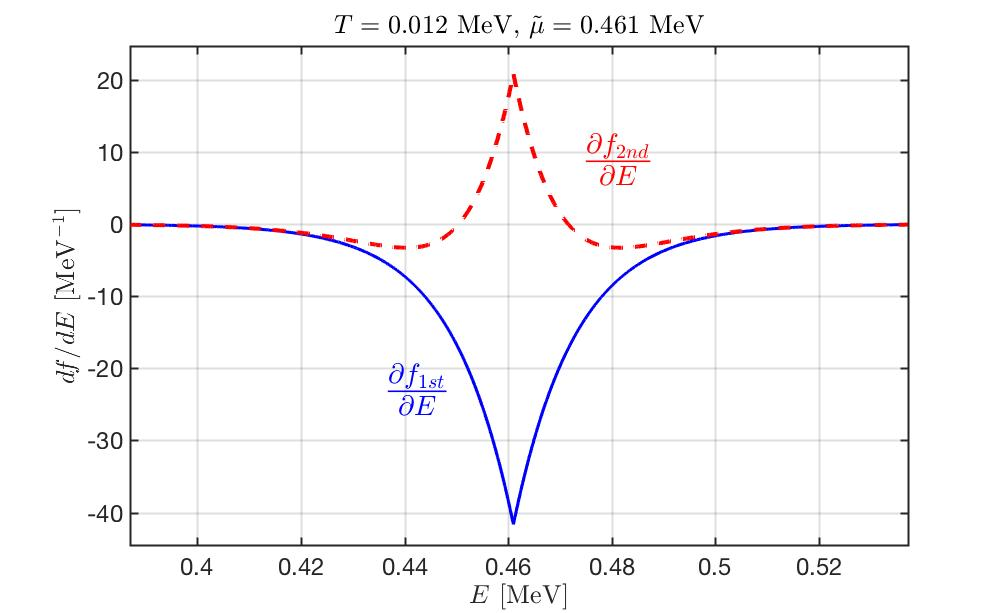
\includegraphics[width=0.9\textwidth]{./plot/dfdE_NovelFermi}
\caption{The $\partial f_{\mathrm{1sr}}/{\partial E}$ and $\partial f_{\mathrm{2nd}}/{\partial E}$ as a function of energy where the parameters are given by $T=0.012\,\mathrm{MeV}$ and chemical potential $\tilde\mu=0.461$ MeV.}
\label{dfdE_fig}
\end{center}
\end{figure}
%~~~~~~~~~~~~~~~~~~~~~~~~~~~~~~~~~~~~~~~~~~~~~~~~~~
%~~~~~~~Figure~~~~~~~~~~~~~~~~~~~~~~~~~~~~~~~~~~~~~
\begin{figure}[ht]
\begin{center}
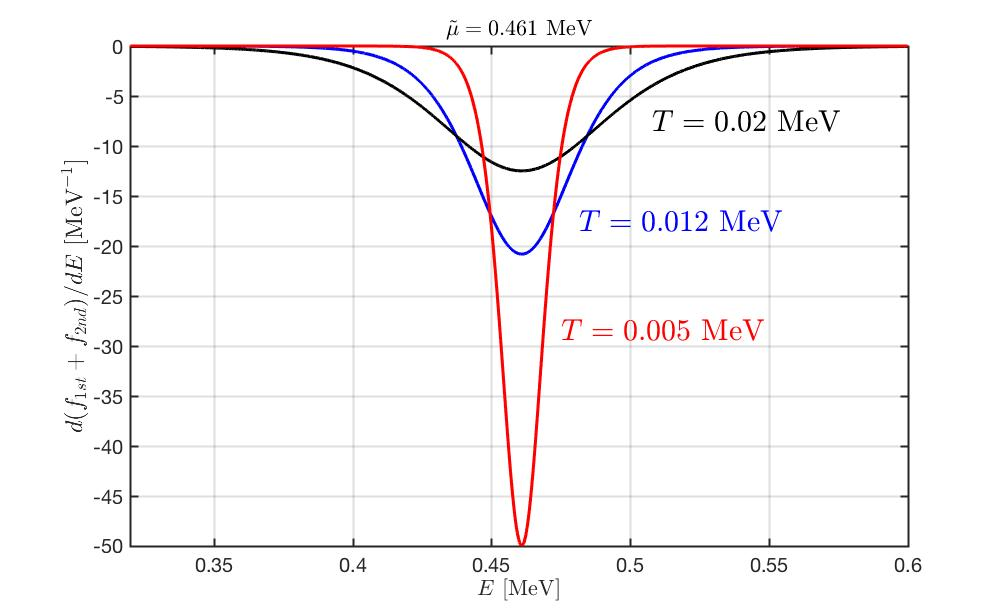
\includegraphics[width=0.9\textwidth]{./plot/dfdE_NovelFermi002}
\caption{
The $d(f_\mathrm{1st}+f_\mathrm{2nd})/dT$ as a function of energy with chemical potential $\tilde\mu=0.461$ MeV.The bule line represents the temperature $T=0.012$ MeV, red line label $T=0.005$ MeV, and black line is $T=0.02$ MeV.}
\label{dfdE_tot_fig}
\end{center}
\end{figure}
%~~~~~~~~~~~~~~~~~~~~~~~~~~~~~~~~~~~~~~~~~~~~~~~~~~



%To demonstrate the benefits of using the novel Fermi distribution form in the calculation of magnetization, we first focus on the function $A_n$ Eq.~(\ref{Function_A}) which contain the derivative of distribution function with respect to energy. We have
%\begin{align}
%A_n=-\int_{m_n}^\infty\!\!&dE_n \frac{\sqrt{E^2_n-m^2_n}}{E_{n}}\delta(\tilde\mu-E_n)\notag\\
%&+\int_{m_n}^\infty\!\!dE_n \frac{\sqrt{E^2_n-m^2_n}}{E_{n}}\frac{e^{-|E_n-\tilde\mu|/T}}{2T}\left[-1+\frac{1-\sinh(|E-\tilde\mu|/T)}{2\cosh^2((E_n-\tilde\mu)/2T)}\right],
%\end{align}
%where the variable $m_n^2=m^2_e+2eBn$.
%and the magnetic susceptibility is given by
%\begin{align}
%    \chi=\frac{\partial M}{\partial B}=\frac{1}{V\beta}\left(\frac{\partial}{\partial B}\frac{\partial \ln Z_{tot}}{\partial B}\right)
%\end{align}

%%%%%%%%%%%%%%%%%%%%%%%%%%%%%%%%%%%%%%%%%%%%%%%%%%%%%%%%%%%%%%%%%



 

\backmatter

\bmhead{Acknowledgments}

We thank Gordon Baym and John W. Clark for their encouragement to publish this result.


\bibliography{sn-bibliography}% common bib file
%% if required, the content of .bbl file can be included here once bbl is generated
%%\input sn-article.bbl


\end{document}
